\chapter*{Week 7: Vectors, Randomness, and Structs}
\addcontentsline{toc}{chapter}{Week 7: Vectors, Randomness, and Structs}
\setcounter{chapter}{8}
\setcounter{section}{0}
% \usepackage{graphicx} % Required for inserting images
% \usepackage{minted}

% \usepackage[LGR, T1]{fontenc}
% \usepackage[utf8]{inputenc}
% \usepackage{textcomp}
% \usepackage{amsthm}
% \usepackage{hyperref}
% \usepackage[margin=1in]{geometry}
% \usepackage[breakable]{tcolorbox}
% \usepackage[cache=false]{minted}





\begin{abstract}
This week will cover:
\begin{enumerate}
    \item Vectors
    \item Randomness
    \item Structs
\end{enumerate}
    
\end{abstract}

\section{Background}

\subsection{Vectors}

Let's start with something we already know about - Arrays.

To recap, an array is a contiguous series that holds a fixed number of values of the same datatype.

A vector is a template class that uses all of the syntax that we used with vanilla arrays, but adds in functionality that relieves us of the burden of keeping track of memory allocation for the arrays. It also introduces a bunch of other features that makes handling arrays much simpler.

First things first. We need to include the appropriate header files to use the vector class.

\mintinline{c++}{#include <vector>}

We can now move on to declaring a vector. This is general format of any vector declaration:

\mintinline{c++}{vector <datatype_here> name(size);}

The size field is optional. Vectors are dynamically-sized, so the size that you give them during initialization isn't permanent - they can be resized as necessary.

You can access elements of a vector in the same way you would access elements in an array, for example array[4]. Remember, indices begin from 0.

The C++ vector class comes with \textcolor{cyan}{\href{https://www.cplusplus.com/reference/vector/vector/vector/}{several member functions}} available in the C++ reference guide, but following are the ones you will need in this week:

\begin{itemize}
    \item \mintinline{c++}{size()} return the size of a vector
    \item \mintinline{c++}{at()} takes an integer parameter for index and returns the value at that position
\end{itemize}

Adding elements to the vector is done primarily using two functions

\mintinline{c++}{push_back()} takes in one parameter (the element to be added) and appends it to the end of the vector. Here is an example:

\begin{example}
    How to use \mintinline{c++}{push_back()} with vectors:

    \begin{minted}{c++}
vector <int> vector1; // initializes an empty vector
vector1.push_back(1); //Adds 1 to the end of the vector. 
vector1.push_back(3); //Adds 3 to the end of the vector. 
vector1.push_back(4); //Adds 4 to the end of the vector. 
cout<< vector1.size(); //This will print the size of the vector - in this case, 3.
// vector1 looks like this: [1, 3, 4]
    \end{minted}
\end{example}

\mintinline{c++}{insert()} can add an element at some position in the middle of the vector.

\begin{example}
    How to use \mintinline{c++}{insert} with vectors:

    \begin{minted}{c++}
// vectorName.insert(vectorName.begin() + position, element)
vector1.insert(vector1.begin() + 1, 2);
cout << vector1.at(1) << endl; // 2 is at index=1
// vector1 looks like this: [1, 2, 3, 4]
    \end{minted}
\end{example}

Here, the \mintinline{c++}{begin} function returns an iterator to the first element of the vector. Due to the nature of an iterator, this allows for the utility of using \mintinline{c++}{begin()} to refer to the first element and \mintinline{c++}{begin()+k} would refer to the kth element in the vector, starting at 0.

Elements can also be removed.

\mintinline{c++}{pop_back()} deletes the last element in the vector.

\begin{example}
    How to use \mintinline{c++}{pop_back()} with vectors:
    \begin{minted}{c++}
vector <int> vector1; // initializes an empty vector
vector1.push_back(1); //Adds 1 to the end of the vector. 
vector1.push_back(3); //Adds 3 to the end of the vector. 
vector1.push_back(4); //Adds 4 to the end of the vector. 
vector1.pop_back(); //Removes the last element of the vector.
//vector1 looks like this: [1, 3]
    \end{minted}
\end{example}

\mintinline{c++}{erase()} can delete a single element at some position, which is shown below using the iterator function of \mintinline{c++}{begin()} to erase the first element of the vector.

\begin{example}
    How to use \mintinline{c++}{erase()} with vectors:

    \begin{minted}{c++}
// vector_name.erase(vector_name.begin() + position)
vector1.erase(vector1.begin() + 0);
cout << vector1.at(0) << endl; //2 is at index=0
// vector1 looks like this: [2, 3, 4]
    \end{minted}
\end{example}

It may be useful to think of vectors relationship to arrays as something similar to strings vs arrays of characters; they are similar concepts, but with added utility and flexibility that is helpful. Vectors are also passed by value (like strings) instead of passed by reference (like arrays). This might look something like:

\begin{example}
    Full vector example:

    \begin{minted}{c++}
void myVecEditFunction(vector <int> vec){
   vec.erase(vec.begin());
   //vec now contains the original vector minus the starting element
}

...

int main(){
   vector <int> originalVector = {1, 2, 3};
   myVecEditFunction(originalVector);
   //originalVector still looks like [1, 2, 3]
}
    \end{minted}
\end{example}

\subsection{Randomness}

Random numbers are a valuable tool for a number of applications, including writing games where we want random chance to be a factor. There are limitations in being able to make a truly random number generator with code, but we have tools to get close enough.

\mintinline{c++}{rand()} function is an inbuilt function in C++ STL, which is defined in header file \mintinline{c++}{<cstdlib>}. \mintinline{c++}{rand()} is used to generate a series of random numbers. The random number is generated by using an algorithm that gives a series of non-related numbers whenever this function is called. The \mintinline{c++}{rand()} function is used in C++ to generate random numbers in the range \mintinline{c++}{[0, RAND_MAX)}.

\mintinline{c++}{RAND_MAX}: It is a constant whose default value may vary between implementations but it is granted to be at least 32767.

The syntax for the function is: \mintinline{c++}{int rand(void);} where \mintinline{c++}{int} is the return type and the parameter list is void (i.e. needs to parameters).

However in order to ensure that the random sequence of numbers is unique each time, we must choose a unique starting seed for the random generator.

\mintinline{c++}{srand()} function is an inbuilt function in C++ STL,  which is defined in \mintinline{c++}{<cstdlib>} header file. \mintinline{c++}{srand()} is used to initialize random number generators. The \mintinline{c++}{srand()} function sets the starting point for producing a series of pseudo-random integers. If \mintinline{c++}{srand()} is not called, the \mintinline{c++}{rand()} seed is set as if \mintinline{c++}{srand(1)} were called at the program start. Any other value for seed sets the generator to a different starting point. 

Here are the two function prototypes for \mintinline{c++}{srand()} to see the syntax:

\begin{minted}{c++}
void srand( unsigned seed );
int srand( unsigned int seed);
\end{minted}

Seeds the pseudo-random number generator used by rand() with the value seed.
Parameter \textbf{seed}: A seed for a new sequence of pseudo-random numbers to be returned by successive calls to rand()

Return value: This function returns a pseudo-generated random number.

\textbf{Note:} The pseudo-random number generator should only be seeded once, before any calls to rand(), and at the start of the program. It should not be repeatedly seeded or reseeded every time you wish to generate a new batch of pseudo-random numbers. 

Standard practice is to use the result of a call to \mintinline{c++}{srand(time(0))} as the seed. However, \mintinline{c++}{time()} returns a \mintinline{c++}{time_t} value which varies every time and hence the pseudo-random number varies for every program call. 

Here are a few examples of using randomness.

\begin{example}
    A short example to roll a die:

    \begin{minted}{c++}
int main(){
    //declare variables
    int dieRoll;
    //random seed 
    srand(time(0));

    dieRoll = rand()%6; //randomly generate a number 0 through 5
    dieRoll+=1; //add 1 to make it now store a number 1 through 6

    //printing a random number stored in a variable
    cout << "Our dice roll is " << dieRoll << endl; 

    //printing the random number directly
    cout << "Our D20 rolled " << rand()%20+1 << endl; 
}
    \end{minted}
\end{example}

\begin{example}
    A long example to play Rock, Paper, Scissors:

    \begin{minted}{c++}
int main(){
    //declare variables
    char userChoice; //to store the user's choice of R, P or S
    int compChoice; //to store the computer's choice
    srand(time(0));

    //ask the user for their choice
    cout << "Rock (R), Paper (P), or Scissors (S)?" << endl;
    cin >> userChoice;

    compChoice = rand()%3; //randomly choose a number 0, 1 or 2

    //Arbitarily choosing that 0 = R, 1 = P, 2 = S for comparison
    switch(userChoice){
        case 'R':
            switch(compChoice){
                case 0: 
                    cout << "Both chose rock-- tie!" << endl;
                    break;
                case 1:
                    cout << "You chose rock, the computer chose ";
                    cout << "paper -- you lose." << endl;
                    break;
                case 2:
                    cout << "You chose rock, the computer chose ";
                    cout << "scissors -- you win!" << endl;
            }
            break;
        case 'P':
            switch(compChoice){
                case 0: 
                    cout << "You chose paper, the computer chose ";
                    cout << "rock -- you win!" << endl;
                    break;
                case 1:
                    cout << "Both chose paper -- tie!" << endl;
                    break;
                case 2:
                    cout << "You chose paper, the computer chose ";
                    cout << "scissors -- you lose." << endl;
            }
            break;
        case 'S':
            switch(compChoice){
                case 0: 
                    cout << "You chose scissors, the computer "; 
                    cout << "chose rock -- you lose." << endl;
                    break;
                case 1:
                    cout << "You chose scissors, the computer "; 
                    cout << "chose paper -- you win!" << endl;
                    break;
                case 2:
                    cout << "Both chose scissors -- tie!" << endl;
            }
            break;
        default:
            cout << "Invalid choice." << endl;
    }

}

    \end{minted}
\end{example}

\subsection{Structs}

In C++, we can define a structure using the keyword struct like so:

\begin{minted}{c++}
struct State
{
    string name;
    int area;
};                   // <-- semicolon after struct definition
\end{minted}

This defines a new type, State, that you can use for declaring variables, e.g.

\begin{minted}{c++}
//create a State variable with no name or area
State emptyState;

//create a State variable with a name and area
State colorado{"Colorado", 104094};
\end{minted}

The variables \mintinline{c++}{emptyState} and \mintinline{c++}{colorado} both have two named attributes, called members - \mintinline{c++}{name} and \mintinline{c++}{area}. We can access each member using dot notation, e.g.

\begin{minted}{c++}
//set members for empty State
emptyState.name = "Texas";
emptyState.area = 268596;

//get members for colorado
cout << colorado.name << " has an area of " << colorado.area << " square miles." << endl;
\end{minted}

Expected output:

\begin{verbatim}
Colorado has an area of 104094 square miles.
\end{verbatim}

If we want to compare two structs, we cannot do so directly. Instead, we must compare each data member individually to see if they match, e.g.

\begin{minted}{c++}
//check each data member by one
if(colorado.name == emptyState.name && colorado.area == emptyState.area)
{
    cout << "These are the same state!" << endl;
}
else
{
    cout << "These are not the same state!" << endl;
}
\end{minted}

Expected output:

\begin{verbatim}
These are not the same state!
\end{verbatim}

\subsubsection{Structs and Classes}

A class can have a struct as a data member, much like how a class could have any other type of data member. It's important to make sure that the class header file (the .h file) can see the definition of the struct. This can be accomplished by defining the struct inside of the .h file, like below:

\begin{minted}{c++}
// filename: example.h
struct State
{
    string name;
    int area;
};                // don't forget the semicolon

class Example
{
    private:
        State my_state_;
        //other data members

    public:
        //setter accepts a State parameter
        void setState(State new_state);

        //getter returns the State member variable
        State getState();

        //other member methods
};
\end{minted}

Any file that includes the .h file shown above will be able to use instances of the State struct, so you will not need to define the State struct anywhere else.

\subsubsection{Vectors of Structs}

Much like how we can have vectors of objects, we can also have vectors of structs. We would define a vector of structs like so:

\begin{minted}{c++}
struct State
{
    string name;
    int area;
};

//create a vector of States
vector<State> my_states;

//add a state to the vector
State new_state{"Random State", 123};
my_states.push_back(new_state);
\end{minted}

\subsubsection{When to use Structs vs Classes}
While structs and classes are similar, there are some key differences between them. When deciding whether you should use one over the other, consider the functionality you'd like to achieve. A good rule of thumb is to ask whether the data type you're defining will need to have any methods or private variables. If it will, then you should create a class. If all members can be public and there are no methods, then a struct may be better.

\section{Warmup}

\problem Spot the error:

\begin{minted}{c++}
#include <vector>
#include <iostream>

// appends the second vector on the first, returns the combined vector
vector<int> appendVectors(vector<int> first, vector<int> second){
    int size = vector.size(second);
    for (int i = 0; i < size; i++){
            first.append(second[i]);
    }
    return second;
}
\end{minted}

\problem Spot the error: 

\begin{minted}{c++}
#include <vector>
using namespace std;

// calls the function from 2.1. Assume 2.1 is already fixed
// prints out the combined vector
int main(){
    vector<int> vect1
    vect1.push_back(10)
    vect1.push_back(20)
    vector<int> vect2;
    vect2.push_back(1);
    vect2.push_back(2);
    cout << appendVectors(vect1, vect2) << endl;
    return 0;
}
\end{minted}

\problem  Let’s print an empty chess board onto the console using structs! There are several errors in the program below relating to how we access the data members of our Tile struct. Identify the errors. 

\begin{minted}{c++}
#include <iostream>
 
using namespace std;
 
struct Tile{
   string piece;
   string tileColor;
};
 
int main(){
   struct Tile board[8][8];
 
   // Color tiles alternately
   for(int i = 0; i < 8; i++){
       for(int j = 0; j < 8; j++){
           if(i % 2 == 0){
               if(j % 2 == 0) board[i][j].getTileColor() = "black";
               else board.tileColor = "white";
           }
           else{
               if(j % 2 == 0) board.getTileColor = "white";
               else board[i][j].tileColor() = "black";
           }
       }
   }
 
   // Print
   for(int i = 0; i < 8; i++){
       for(int j = 0; j < 8; j++){
           if(board[i][j].tileColor() == "black") cout << "▒";
           else cout << " ";
       }
       cout << "\n";
   }
}
\end{minted}

\problem Now we'll populate one side of the chess board with the unicode characters for chess pieces. This code also has errors, identify them:

\begin{minted}{c++}
#include <iostream>
 
using namespace std;
 
struct Tile{
   string piece;
   string tileColor;
};
 
int main(){
   struct Tile board[8][8];
 
   // Color tiles alternately
   for(int i = 0; i < 8; i++){
       for(int j = 0; j < 8; j++){
           board[i][j].piece = "none";
           if(i % 2 == 0){
               if(j % 2 == 0) board[i][j].tileColor = "black";
               else board[i][j].tileColor = "white";
           }
           else{
               if(j % 2 == 0) board[i][j].tileColor = "white";
               else board[i][j].tileColor = "black";
           }
       }
   }
 
   // populate one side of the chess board
   board[0][0].piece() = "♜";
   board[0][1].piece() = "♞";
   board[0][2].piece() = "♝";
   board[0][3].piece() = "♛";
   board[0][4].piece() = "♚";
   board[0][5].piece() = "♝";
   board[0][6].piece() = "♞";
   board[0][7].piece() = "♜";
 
   for(int i = 0; i < 8; i++) board[1][i].setPiece("♟");
 
   // Print
   for(int i = 0; i < 8; i++){
       for(int j = 0; j < 8; j++){
           if(!board[i][j].piece.compare("none")){
               if(board[i][j].tileColor == "black") cout << "▒";
               else cout << " ";
           }
           else{
               cout << board[i][j].piece;
           }
       }
       cout << "\n";
   }
}
\end{minted}



\problem The following program is intended to generate a random number between 1 and 32 inclusively. Fill in the blanks:

\begin{minted}{c++}
#include<iostream>
#include<cstdlib>
#include<ctime>
using namespace std;

int main() 
{
    // Fill the line below to make the generated random number different for each run.
    _____________________________________
    int random_number = 0;
    // Fill the line below to generate a random number between 1 to 32 inclusively.
    _______________________________
    cout << "Number generated is " << random_number << endl;
    return 0;
}

\end{minted}

\section{Recitation}

\subsection{Working with Vectors}
In this problem, you will write a program to

\begin{itemize}
    \item accepts 20 floating point values from the user and store them in a vector
    \item find the average of all the values in the vector
    \item remove all elements that are more than the calulated average
\end{itemize}

Each of these three requirements should be implemented in individual functions. The parameters and return types of these functions are up to you. The full solution should consist of a `main' function which drives the program, using the three functions written for each sub-task and outputting the result at each stage. 

\begin{multipart}
Write three algorithms in pseudocode for the three tasks above.
\end{multipart}

\vspace{6cm}

\begin{multipart}
Imagine how a sample run of your program would look like. Think about at least two examples.
\end{multipart}

\vspace{6cm}

\begin{multipart}
Identify the values that you must test for. We call these values ``boundary conditions”.
\end{multipart}

\vspace{6cm}

Implement your solution in C++ using VS Code. Revise your solution, save, compile and run it again. Are you getting the expected result and output? Keep revising until you do. Make you sure you test for the values used in your sample runs, and for the boundary conditions. Paste your code in the Recitation assignment.

\subsection{Working with Probability}
You’re playing darts with an oddly-shaped dart board. The board is in the shape of a square, with a shaded circle somewhere inside it. The size of the circle is randomly generated, but you know its radius will be smaller than ½ the length of one side of the square.

Every time you throw a dart, assume that you are guaranteed to land inside the square, but you have an equal chance of landing anywhere inside it.

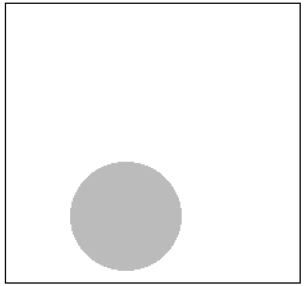
\includegraphics{images/rec12.png}

Write a function that accepts a single parameter, \mintinline{c++}{double side_length}. This will be the length of one side of the square. Then, your function should randomly generate a radius for the circle, which must be less than \mintinline{c++}{(side_length/2)}. Print this radius: \mintinline{c++}{"The radius of the circle is: ."} Finally, calculate the probability of landing in the circle if you throw one dart (which is equally likely to hit anywhere in the square). Print this value as a double between 0 and 1. \mintinline{c++}{"The probability of landing in the circle is: "}

You should also write a main function which prompts the user to input a value for the side length of the square. Make sure that this value is appropriate (i.e. a positive number), and then pass the value to your newly-written function.

Formulas:

\begin{verbatim}
Area of a square: side_length²
Area of a circle: pi * radius²
Use 3.14 as the value of pi
\end{verbatim}

Example output (red is user input):

\begin{sample}
Enter side length: \textcolor{red}{10}

The radius of the circle is: 3.21

The probability of landing in the circle is: 0.323548
\end{sample}

\begin{multipart}
Write an algorithm in pseudocode for the program above.
\end{multipart}

\vspace{6cm}

\begin{multipart}
Imagine what a sample run of your program would look like.
\end{multipart}

\vspace{6cm}

\begin{multipart}
 Identify the values that you must test for. We call these values ``boundary conditions".
\end{multipart}

\vspace{6cm}

\begin{multipart}
Implement your solution in C++ using VS Code. Revise your solution, save, compile and run it again. Are you getting the expected result and output? Keep revising until you do. Make you sure you test for the values used in your sample runs, and for the boundary conditions. Paste your code in the recitation assignment.
\end{multipart}

